% JAWS 2 @ ASE 2026 — Idea Paper (≤8 pages excl. references)
% ACM Primary Article Template, sigconf, single-anonymous
\PassOptionsToPackage{expansion=false}{microtype}
\documentclass[sigconf,nonacm]{acmart}

% JAWS is single-anonymous: author names visible
\settopmatter{authorsperrow=3}

\usepackage{booktabs}
\usepackage{multirow}
\usepackage{xcolor}
\usepackage{tikz}
\setlength{\headheight}{16.36pt}
\setcounter{topnumber}{3}
\renewcommand{\topfraction}{0.95}
\usetikzlibrary{arrows.meta,positioning,calc,decorations.pathreplacing}

% Blind-review off (single-anonymous)
\setcopyright{none}
\renewcommand\footnotetextcopyrightpermission[1]{}
\pagestyle{plain}

\title{From Symptom to Structure: Analyzing Disagreement\\in Agent-Skill Security Scanners}




\begin{abstract}
Automated security analyses routinely disagree, yet evaluations treat that disagreement as a statistic (Cohen's $\kappa$, pairwise overlap) and stop there, as if it were noise or merely an outcome about tool quality.
We propose to treat disagreement differently: as \emph{analytical evidence about the analyses themselves}.
The structure of disagreement, once made comparable, exposes each analysis's coverage of the threat space and how it operationalizes detection there.
We develop a methodology for this conversion: a shared observation language that makes disagreement localizable, a three-layer decomposition: a miss can originate in \emph{coverage} (the input was never collected), \emph{detection} (the engine cannot recognize it), or \emph{decision} (the finding was thresholded away); blind-spot hypotheses locked before construction, and adversarial validation.
We instantiate the idea on agent-skill security scanners, an emerging supply-chain defense whose scanners disagree sharply.
Across 581 malicious skills (350 wild, 231 coordinate-generated) and three heterogeneous scanners, the decomposition predicts concrete blind spots, and locked adversarial construction confirms them: hidden-file payloads evade SkillSpector on 14/15, finding-family variants evade Cisco on 6/6, and combined strategies evade SkillSpector on 5/5, with selected failures traced to source-level mechanisms.
Disagreement, we argue, is not merely a statistic to report: it is evidence to mine.
\end{abstract}

\keywords{agent skills, security scanners, disagreement analysis, blind spots, adversarial construction}

\begin{document}
\maketitle

% ============================================================
\section{Introduction}
\label{sec:intro}

Automated security analyses disagree.
Given the same artifact, one scanner flags it, another passes it, and a third flags something else entirely.
The standard response is to \emph{measure} the disagreement (Cohen's $\kappa$, pairwise overlap, per-tool recall) and treat the result as an evaluation outcome: a fact about tool quality, or noise to be averaged away.
We ask a different question: \emph{what does the pattern of disagreement reveal about the analyses themselves?}
We argue that disagreement is not merely a statistic to report.
It is analytical evidence: once disagreements are made comparable, their structure exposes what each analysis covers, what it cannot see, and why.

Today this evidence is inaccessible, because analyses speak incompatible languages.
One scanner reports ``tool poisoning,'' another ``supply-chain risk,'' a third a family of regex matches.
There is no shared frame in which to ask \emph{where exactly} they disagree, so disagreement remains global (a $\kappa$) but never localizable.
Without localization there is no explanation; without explanation, disagreement cannot be acted upon.

We propose to convert disagreement into structure.
The conversion has four steps.
First, a \emph{shared observation language} (a coordinate space over the threat space) into which each scanner's categories are mapped, making disagreement localizable.
Second, a \emph{three-layer decomposition}: every miss originates in exactly one architectural layer: \emph{coverage} (the input was never collected), \emph{detection} (the engine cannot recognize the behavior), or \emph{decision} (the finding exists but is thresholded away).
Third, the decomposition yields \emph{blind-spot hypotheses}, which we lock before building anything.
Fourth, \emph{adversarial validation}: coordinate-driven construction tests the locked hypotheses, and selected failures are traced to implementation mechanisms.

We instantiate this idea on \emph{agent-skill security scanners}.
Coding agents extend their capabilities by installing skills (packages of instructions and scripts), and malicious skills are a live supply-chain threat (the ClawHavoc incident surfaced over 1{,}184 of them~\cite{clawhub2026}).
Scanners have emerged to screen skills, but they disagree sharply~\cite{clawhub2026,locatejudge2026}, and no existing evaluation explains the disagreement.
The object is timely; the methodology is the contribution.

An honesty point frames our results.
In aggregate the scanners are strong: across 581 malicious skills, SkillSpector flags 92.9\%, Cisco 86.7\%, Caterpillar 72.6\% under a uniform reading of their outputs (any surfaced finding counts; operationalized in Table~\ref{tab:disagg}).
The blind spots are therefore invisible in average recall; they emerge only when the threat space is partitioned.
This is precisely the structure that aggregate metrics conceal, and precisely what disagreement, treated as evidence, exposes.

\noindent\textbf{Contributions.} Three, in strict hierarchy:
\begin{itemize}
  \item \textbf{Core idea.} Disagreement among automated security analyses is not merely an evaluation outcome: projected into a shared observation space, its structure becomes evidence about the analyses themselves, from which falsifiable blind-spot predictions can be derived.
  \item \textbf{Methodology.} A loop converting disagreement into such predictions: observe where scanners disagree, decompose why (coverage, detection, decision), lock what they will miss next, and test whether the prediction holds.
  \item \textbf{Demonstration.} An end-to-end instantiation on agent-skill security scanners: 581 malicious skills, 500 benign references, three scanners, six locked hypotheses with confirmed, partial, and rejected outcomes, traced to source-level mechanisms.
\end{itemize}

\noindent\textbf{Scope.} We demonstrate the loop end-to-end on one instantiation.
The generality of the idea (package scanners, dependency scanners, static analyzers, LLM-based security evaluators) is the research direction this early result opens, to be developed in an extended version.

\noindent\textbf{Results.} The loop's predictions held where its evidence was architectural: locked hypotheses predicted hidden-file evasion of SkillSpector (observed 14/15), regex blindness to semantic phrasing (10/10), and Cisco's failure on finding-family variants (6/6); one hypothesis was partially confirmed and one rejected by its own control experiment. Each confirmed prediction traces to a named source-level mechanism. The bypasses are not the contribution; they are the evidence that the conversion works.

% ============================================================
\section{The Core Idea: Disagreement as Evidence}
\label{sec:idea}

An automated security analysis is a pipeline: it \emph{collects} an input, \emph{detects} patterns in it, and \emph{decides} what to report. Each stage can fail independently, and the stages fail differently across analyses. This gives the paper's central object a precise shape:

\medskip\noindent\textbf{Three-layer decomposition.} Every miss originates in one layer, or in a short chain through adjacent layers: \emph{L1 coverage} (the relevant input was never collected), \emph{L2 detection} (the input was collected but the engine cannot recognize the behavior), \emph{L3 decision} (the engine produced a finding but the decision rule discarded it).\medskip

The layers are not metaphorical; they are separable by construction. A payload placed in a file the collector skips evades at L1 regardless of engine strength. A behavior expressed without the lexical or semantic surface an engine matches evades at L2. A finding demoted below a severity threshold evades at L3. Each layer implies a different fix (collect more inputs; change engines; change thresholds), a different attack strategy (hide the file; change the expression; suppress the severity), and therefore a different falsifiable blind-spot hypothesis.

The paper's progression is the same ladder: the observation space answers \emph{where} scanners disagree (\S\ref{sec:measure}), the three layers answer \emph{why} (\S\ref{sec:explain}), locked hypotheses answer \emph{what they will miss next} (\S\ref{sec:hypotheses}), and construction answers \emph{whether the prediction is true} (\S\ref{sec:validate}). Why is a new instrument needed to climb it? Because the standard tools operate at the wrong level of aggregation (Table~\ref{tab:why}):

\begin{table}[t]
\caption{What each approach can do with disagreement. ``Localize'' = say where in the threat space the disagreement arises; ``explain'' = attribute it to a mechanism in the analysis; ``predict'' = derive the failure before any new artifact is built.}
\label{tab:why}
\small
\begin{tabular}{@{}lccc@{}}
\toprule
 & Localize & Explain & Predict \\
\midrule
Aggregate recall & $\times$ & $\times$ & $\times$ \\
Pairwise $\kappa$ / overlap & $\times$ & $\times$ & $\times$ \\
Manual post-hoc audit & \checkmark & \checkmark & $\times$ \\
\textbf{Our loop} & \checkmark & \checkmark & \checkmark\ (locked) \\
\bottomrule
\end{tabular}
\end{table}

Recall and $\kappa$ compress disagreement to a scalar; scalar differences cannot say \emph{where} the analyses diverge. A manual audit can, after seeing the failures; but post-hoc explanation cannot distinguish prediction from rationalization. The loop we instantiate (observe, localize, decompose by layer, hypothesize, lock, construct, validate) is the minimal pipeline that does all three, and its predictions are checkable against a locking protocol that fixes hypotheses before construction.

% ============================================================
\section{An Observation Instrument}
\label{sec:measure}

The reason disagreement cannot currently be interrogated is that the scanners speak incompatible languages: SkillSpector speaks of 17 risk classes, Cisco of 18 threat categories, Caterpillar of regex rule families. There is no frame in which to ask \emph{where exactly} they disagree. The coordinate space we introduce is, first and foremost, a \emph{shared observation language}: the instrument that makes disagreement localizable. It is not a universal taxonomy; it is the observation layer required to interrogate disagreement. Figure~\ref{fig:pipeline} shows the full conversion this paper instantiates.

\begin{figure*}[t]
\centering
\resizebox{\textwidth}{!}{\begin{tikzpicture}[node distance=4mm and 7mm,
  box/.style={draw=black!40, rounded corners=1pt, font=\footnotesize, align=center, inner sep=3pt},
  plain/.style={font=\footnotesize, align=center},
  arrow/.style={-{Stealth[length=2mm]}, thick, black!60},
  inflow/.style={draw, rounded corners=1pt, font=\footnotesize, align=center, inner sep=3pt, fill=black!5}]

% ============ LEFT: current practice ============
\node[plain, font=\footnotesize\bfseries, black!55] (lp) at (0,4.35) {CURRENT PRACTICE};
% ---- left panel: fixed coordinates, total width <= 57mm ----
\node[inflow, minimum width=15mm] (art) at (0,1.6) {artifact $X$};
\node[inflow, minimum width=15mm] (sa) at (2.7,2.7) {Scanner A};
\node[inflow, minimum width=15mm] (sb) at (2.7,1.6) {Scanner B};
\node[inflow, minimum width=15mm] (sc) at (2.7,0.5) {Scanner C};
\draw[arrow] (art.east) -- (sa.west); \draw[arrow] (art.east) -- (sb.west); \draw[arrow] (art.east) -- (sc.west);
\node[plain] at (4.35,2.7) {$\checkmark$};
\node[plain] at (4.35,1.6) {$\times$};
\node[plain] at (4.35,0.5) {$\times$};
\node[box, fill=black!5, minimum width=13mm] (kap) at (6.1,1.6) {$\kappa$, overlap};
\draw[arrow] (4.8,1.6) -- (kap.west);
\node[box, below=3.5mm of kap, fill=black!12, text width=30mm] (stop) {``they disagree.''\\ \emph{Evaluation ends here.}};
\draw[arrow] (kap) -- (stop);

% ============ RIGHT: our view (starts x=6.6cm; no overlap with left) ============
\node[inflow, minimum width=15mm] (art2) at (7.3,1.6) {artifact $X$};
\node[box, fill=blue!8, text width=20mm] (coord) at (9.6,1.6) {\textbf{observation space}\\ $(s,m,t)$ coordinate};
\draw[arrow] (art2) -- (coord);
\node[box, fill=orange!12, text width=20mm] (l1) at (12.1,2.7) {\textbf{L1 coverage}\\ did it collect the input?};
\node[box, fill=orange!12, text width=20mm] (l2) at (12.1,1.6) {\textbf{L2 detection}\\ can the engine see it?};
\node[box, fill=orange!12, text width=20mm] (l3) at (12.1,0.5) {\textbf{L3 decision}\\ is the finding kept?};
\draw[arrow] (coord.east) -- (l1.west);
\draw[arrow] (coord.east) -- (l2.west);
\draw[arrow] (coord.east) -- (l3.west);
\node[box, fill=white, inner sep=3pt] (diag) at (14.9,1.6) {\footnotesize
\begin{tabular}{@{}lccc@{}}
 & \textbf{L1} & \textbf{L2} & \textbf{L3} \\[-1pt]
\textbf{SS} & \textcolor{blue!70!black}{ok} & \textcolor{blue!70!black}{ok} & \textcolor{blue!70!black}{ok} \\[1.5pt]
\textbf{Cisco} & \textcolor{blue!70!black}{ok} & \textcolor{orange!85!black}{literal} & \textcolor{orange!85!black}{drops} \\[1.5pt]
\textbf{Cat} & \textcolor{blue!70!black}{ok} & \textcolor{orange!85!black}{regex} & \textcolor{orange!85!black}{no rule} \\
\end{tabular}};
\draw[arrow] (l1.east) -- (diag.west);
\draw[arrow] (l2.east) -- (diag.west);
\draw[arrow] (l3.east) -- (diag.west);
\node[box, fill=blue!8, text width=44mm] (hyp) at (14.9,-0.7) {\textbf{blind-spot hypothesis per scanner, per layer}};
\draw[arrow] (diag.south) -- (hyp.north);
\node[box, fill=green!10, text width=44mm] (val) at (14.9,-1.9) {\textbf{locked construction $\rightarrow$ validation $\rightarrow$ mechanism}};
\draw[arrow] (hyp) -- (val);
\node[plain, font=\footnotesize\bfseries, black!55] at (9.6,4.35) {OUR VIEW};
\end{tikzpicture}}
\caption{\textbf{The same disagreement, read two ways.} Current practice collapses three verdicts on artifact $X$ into a scalar and stops. Our view localizes $X$ in a shared observation space, decomposes each scanner's failure into one architectural layer (coverage L1, detection L2, or decision L3), derives per-scanner blind-spot hypotheses, and validates them by construction locked before the fact.}
\label{fig:pipeline}
\end{figure*}

\begin{table}[t]
\caption{The three-dimensional observation language. Each threat is a coordinate $(source, mechanism, target)$; all three axes are multi-valued.}
\label{tab:dims}
\small
\begin{tabular}{@{}p{1.2cm}p{1.9cm}p{4.6cm}@{}}
\toprule
Dimension & Question & Values (abbreviated) \\
\midrule
source & where does it enter? & supply chain; user input; external untrusted content; runtime environment; unknown \\
mechanism & how does it attack? & code execution; instruction manipulation; dependency manipulation; privilege abuse; obfuscation; state corruption; \ldots \\
target & what does it seek? & information theft; persistent control; resource abuse; system damage; financial theft; content-safety harm; defense evasion \\
\bottomrule
\end{tabular}
\end{table}

\subsection{Three Dimensions}
Each threat is located by three dimensions (Table~\ref{tab:dims}): \emph{source} (where it enters: supply chain, user input, external untrusted content, runtime environment, or unknown), \emph{mechanism} (how it attacks: code execution, instruction manipulation, dependency manipulation, privilege abuse, obfuscation, state corruption, \ldots), and \emph{target} (what it seeks: information theft, persistent control, resource abuse, system damage, financial theft, content-safety harm, defense evasion). The axes follow established security modeling: the attacker model (cf.\ Dolev--Yao), the technique axis (cf.\ ATT\&CK), and the security-property axis (cf.\ the CIA triad).

\subsection{Mapping Scanner Languages}
We mapped the documented category systems of six scanners (SkillSpector, Cisco, Snyk, Socket, ATH, AARTS; 168 threat categories in total) into the space; the occupied cells consolidate into 43 distinct threat coordinates. The mapping is single-annotator at this stage; measuring its inter-annotator reliability is part of the extended benchmark this idea paper argues for. The mapping is manual and evidence-based: each native category (e.g.\ Cisco's ``tool poisoning,'' SkillSpector's 17 risk classes, Caterpillar's rule families) is assigned to the set of coordinates its triggering conditions actually observe, with multi-valued assignment when a category spans several coordinates; a credential-harvesting rule, for instance, covers any (source $\times$ code execution $\times$ information theft) cell regardless of how the credential was reached. This is where ``semantic alignment'' becomes checkable: two categories from different scanners that map to overlapping coordinate sets are nominally the same detector, and any residual disagreement between them is operational, not semantic. To check that the space can carry existing threat descriptions, we mapped 1{,}253 threat statements from 84 sources. Only 17.9\% map cleanly to a full triple; \textbf{56.5\% are partial triples}: existing vocabularies cannot even fully express them, 5.3\% are compound, and 20.3\% fall into genuine gaps. This partial-triple rate is our key measurement-space evidence: current categorizations do not provide a complete description; a coordinate space does.

\subsection{Orthogonality}
The dimensions carry complementary information: on an 81-category human-verified gold standard, pairwise normalized mutual information stays moderate (0.23--0.57), no axis is redundant (removing any one collapses its 31 occupied coordinates to 15--23), and its 81 native labels compress into 31 coordinates ($2.6\times$) as synonymous scanner vocabularies merge while distinctions survive. The point of the space is not taxonomic completeness; its role here is \emph{inferential}: once scanner outputs are projected into a common coordinate system, disagreement becomes evidence from which hypotheses about missing coverage and operational boundaries can be derived, the input to everything that follows.

% ============================================================
\section{Instantiation: Agent-Skill Scanners}
\label{sec:background}

Agent skills are distributed through marketplaces such as ClawHub and skills.sh~\cite{clawhub2026}; at scale, a snapshot of 138{,}133 public SKILL.md files found 91.8\% exhibiting at least one packaging or safety defect~\cite{reusability2026}, and field measurements attribute 26.1\% of 31{,}132 wild skills with at least one security vulnerability~\cite{skillscan2026}. Because a skill can carry arbitrary instructions and scripts, it is an active supply-chain attack surface: the ClawHavoc incident identified over 1{,}184 malicious skills in a single marketplace~\cite{clawhub2026}, and injected skill instructions achieve up to 80\% attack success on frontier agents~\cite{skillinject2026}. Security scanners have emerged to screen skills before installation~\cite{locatejudge2026}.

We study three scanners spanning the mainstream detection architectures (Table~\ref{tab:scanners}). \textbf{SkillSpector} (NVIDIA) combines static rules, AST analysis, YARA signatures, and an LLM semantic layer. \textbf{Cisco Skill Scanner} (AI Defense) combines static analysis, YARA, LLM-based judgment, and behavioral dataflow. \textbf{Caterpillar} is a lightweight regex-based tool. SkillSpector and Cisco are production-grade; Caterpillar serves as a lower-bound reference showing how blind spots deepen as detection grows more primitive. The three decision rules already preview the operational divergence that \S\ref{sec:explain} measures: a numeric risk score, a severity threshold, and a lexical grade.

\begin{figure}[t]
\centering
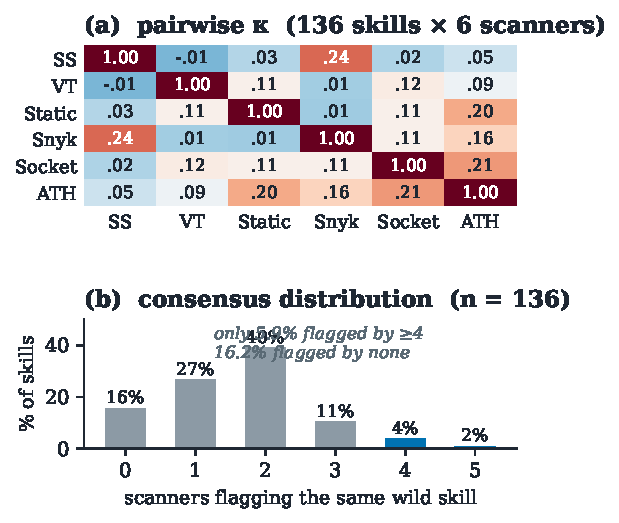
\includegraphics[width=\columnwidth]{fig_census.pdf}%
\Description{Two stacked panels: a six-by-six heatmap of pairwise kappa values, all at most 0.24, and a bar chart of consensus showing most skills flagged by zero to two scanners.}
\caption{\textbf{Disagreement is the norm in the wild.} A market census (project week-0 data, no ground truth; its six scanners overlap with \S\ref{sec:explain}'s three only in SkillSpector): on 136 skills verified across platforms, every pair of public scanners agrees at $\kappa\le 0.244$, most near zero. Consensus is equally scarce: only 5.9\% of skills are flagged by four or more scanners, and on the full 1{,}082-skill census 260 of 445 flagged skills are flagged by exactly one. Disagreement at this scale is not noise to average away; it is the ecosystem's default output.}
\label{fig:census}
\end{figure}

\begin{table}[t]
\caption{The three studied scanners. ``Decision rule'' is what the raw output reduces to for an allow/block decision: each rule is later implicated in a distinct blind spot.}
\label{tab:scanners}
\small
\begin{tabular}{@{}p{1.5cm}p{2.6cm}p{3.6cm}@{}}
\toprule
Scanner & Layers & Decision rule \\
\midrule
SkillSpector & static rules, AST, YARA, LLM semantic & risk score (0--100); $>$50 = detected \\
Cisco & static, YARA, LLM judgment, dataflow & safe unless a CRITICAL/HIGH finding exists \\
Caterpillar & regex families & letter grade; $\neq$A = flagged \\
\bottomrule
\end{tabular}
\end{table}

\begin{table}[t]
\caption{Four corpora, four roles. Each row is a distinct evidential unit; no number crosses rows. Census scanners: SkillSpector, Snyk, Socket, ATH, VirusTotal, static analysis. Main-loop scanners: the three of Table~\ref{tab:scanners}.}
\label{tab:datasets}
\small
\begin{tabular}{@{}p{2.7cm}p{1.5cm}p{3.6cm}@{}}
\toprule
Corpus & $n$ & Role in this paper \\
\midrule
Market census (wild, unlabeled) & 1{,}082 & Motivation: disagreement is pervasive (Fig.~\ref{fig:census}) \\
Malicious corpus & 581 & Observed disagreement: 350 wild + 231 generated by occupied coordinate \\
Benign references & 500 + 4{,}000 & False-positive mirror (500 in-corpus; 4{,}000 official MalSkillBench audit) \\
Constructions & 129 (79 conf.) & Prediction validation: Arms 7--13 locked; 1--6 exploratory; disjoint from the corpus above \\
\bottomrule
\end{tabular}
\end{table}

\textbf{Threat model.} The attacker authors and publishes a skill that a user (or an agent acting for the user) installs from a marketplace. The skill may contain natural-language instructions in SKILL.md, arbitrary scripts, and metadata declarations; everything is readable, but nothing is executed at install time. The defender runs one or more scanners over the skill \emph{before} execution and must decide allow/block with no runtime evidence. The attacker's goal is not to exploit a parser bug but to place malicious behavior where the defender's analysis does not look: outside the scanned file set, outside the literal command surface, or inside a declared capability. All blind spots we report are of this placement kind: architectural, not cryptographic.

These scanners frequently disagree on the same skill. Recent measurements quantify the disagreement: across 67{,}453 skills, pairwise overlap of flagged sets is at most 10.4\%, and only 0.69\% are flagged by all scanners~\cite{clawhub2026}. Yet such numbers stay descriptive: they tell us \emph{that} scanners disagree, not \emph{where} in the attack space the disagreement arises or \emph{why}.

% ============================================================
\section{Observed Disagreement, Layer by Layer}
\label{sec:explain}

With a common observation layer in place, we project each scanner's detections onto the coordinate space and compare scanners coordinate by coordinate. This is the paper's core analysis, measured on 581 malicious skills (350 wild samples stratified by behavior, 231 coordinate-generated) plus 500 benign marketplace skills as a false-positive reference, under one decision rule fixed before analysis.

\subsection{Aggregate Detection Conceals the Structure}
Table~\ref{tab:disagg} shows what the aggregate view sees, and what it hides. Under the uniform reading, SkillSpector flags 92.9\%, Cisco 86.7\%, Caterpillar 72.6\% of the 581 malicious skills (wild 350: 91.1/88.0/70.9; generated 231: 95.7/84.8/75.3, per-class detail in Fig.~\ref{fig:disagg}c). Under each product's \emph{shipped} decision rule the same raw outputs yield 46.8\%, 71.6\%, and 38.6\%: the disagreement statistics are functions of thresholds, not only of scanners. Stopping at any of these numbers, one concludes detection is largely solved or largely broken depending on the rule chosen. The structure emerges one level down (Fig.~\ref{fig:disagg}b): 222 skills (38.2\%) are missed by at least one scanner, and when two agree the third is the sole miss (Caterpillar 118, Cisco 40, SkillSpector 17); and across the 13 wild behavior classes, per-class detection spans 0--100\% (Fig.~\ref{fig:surface}).

\begin{table}[t]
\caption{Observed disagreement under one reproducible decision rule fixed before analysis: Cisco flagged iff \texttt{is\_safe=false} or any MEDIUM-or-higher finding; SkillSpector iff risk score $>0$; Caterpillar iff any finding. Cisco returned null verdicts on 17 malicious skills (counted as non-detections); SkillSpector completed all 581. ``Shipped rules'' rows show what the same raw outputs say under each product's own threshold (Cisco CRITICAL/HIGH; SkillSpector score $>50$; Caterpillar grade $\neq$A). Benign reference: 500 marketplace skills, unaudited; flag rates are upper bounds on false positives.}
\label{tab:disagg}
\small
\begin{tabular}{@{}lrrr@{}}
\toprule
\multicolumn{4}{l}{\emph{(a) Detection rate by subset}} \\
Subset & Cisco & SkillSpect. & Caterp. \\
\midrule
Malicious (581), uniform rule & 86.7\% & 92.9\% & 72.6\% \\
\quad same outputs, shipped rules & 71.6\% & 46.8\% & 38.6\% \\
Benign ref.\ (500), uniform rule & 35.2\% & 44.2\% & 28.6\% \\
\quad same outputs, shipped rules & 11.2\% & 2.8\% & 16.4\% \\
\midrule
\multicolumn{4}{l}{\emph{(b) Pairwise consensus (third scanner is the sole miss)}} \\
Pair flags & $n$ & sole miss & \\
\midrule
Cisco + SkillSpector & 118 & Caterpillar & \\
SkillSpector + Caterpillar & 40 & Cisco & \\
Cisco + Caterpillar & 17 & SkillSpector & \\
Single-scanner flags & 39 & SS 23 / Cisco 10 / Cat 6 & \\
\bottomrule
\end{tabular}
\end{table}

\begin{figure*}[t]
\centering
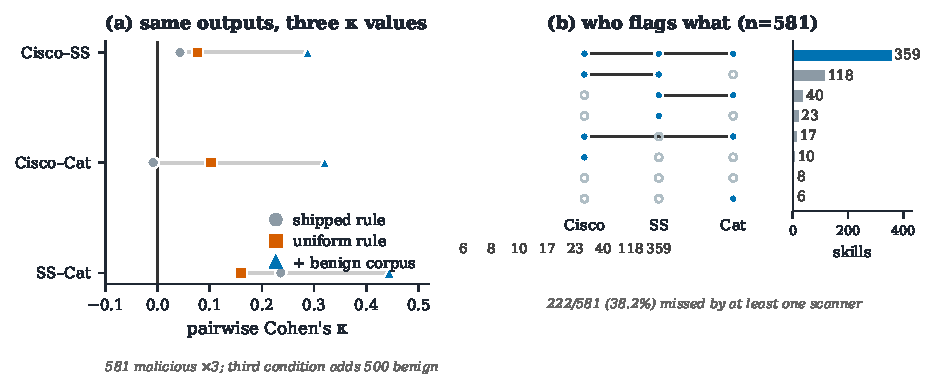
\includegraphics[width=0.87\textwidth]{fig_disagreement.pdf}%
\Description{Left: dot-range plot of pairwise kappa under three rules spanning minus 0.01 to plus 0.44. Right: UpSet matrix of flag combinations with all-three 359 dominant.}
\caption{\textbf{The aggregate view, dismantled.} (a)~Pairwise Cohen's $\kappa$ from the \emph{same} $581{\times}3$ raw outputs under three corpus/rule choices: the statistic swings from $-0.01$ to $+0.44$; no scalar in this range localizes the disagreement. (b)~Flag combinations: misses concentrate in reproducible patterns (Caterpillar sole miss: 118), not noise. Where those misses live in the threat space is Fig.~\ref{fig:surface}'s question.}
\label{fig:disagg}
\end{figure*}

\subsection{The Statistic Itself Is Unstable}
Figure~\ref{fig:disagg}a computes pairwise Cohen's $\kappa$ from the \emph{same} $581\times3$ raw outputs under three defensible choices: malicious-only with shipped rules ($-0.01$ to $+0.24$), malicious-only with the uniform rule ($+0.08$ to $+0.16$), malicious-plus-benign with the uniform rule ($+0.29$ to $+0.44$). The benign corpus dominates the third condition because agreement on easy negatives inflates $\kappa$; the shipped-rule condition collapses because thresholds disagree more than detections do. No scalar in this range says \emph{where} the scanners differ or \emph{why}; the rest of the paper supplies the missing structure.

\begin{figure}[t]
\centering
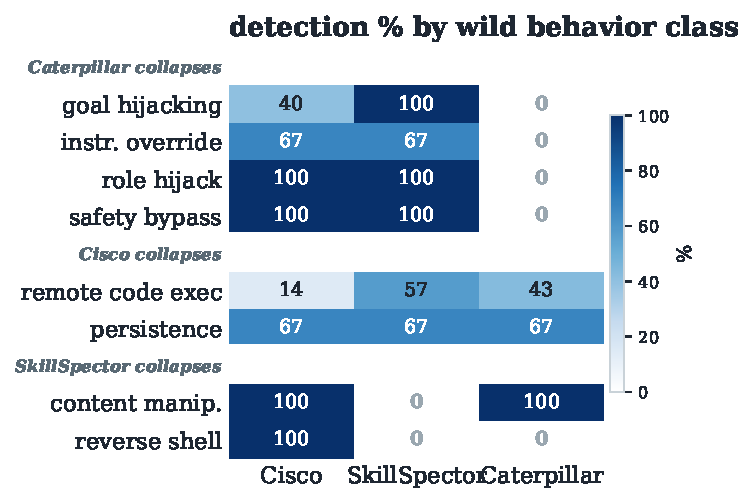
\includegraphics[width=\columnwidth]{fig_surface.pdf}%
\Description{Heatmap of thirteen wild behavior classes by three scanners, grouped into bands by which scanner collapses.}
\caption{\textbf{Localized detection surface: disagreement is structured.} Detection rate per wild behavior class (uniform rule, $n$ in labels), sorted by which scanner collapses rather than by frequency; classes all three hold (malware delivery, privilege escalation, credential theft, data exfiltration, resource abuse) are omitted. Three scanner-specific failure bands appear: Caterpillar on instruction-level classes, Cisco on deep-disguise RCE, SkillSpector on content manipulation and reverse shell; above them, a base of classes all three hold. An aggregate recall number averages over these bands and erases them.}
\label{fig:surface}
\end{figure}

\subsection{L1: Coverage Failures}
A coverage failure is architectural: the scanner does not inspect the region at all. Figure~\ref{fig:surface} localizes them empirically: all 13 wild behavior classes, sorted not by frequency but by \emph{which scanner collapses}: Caterpillar folds on instruction-level classes (goal hijacking, instruction override: 0\%); Cisco folds on deep-disguise remote code execution (14\%); SkillSpector folds on content manipulation and reverse shell (0\%), while the mass of the corpus (malware delivery) is held by all three. The canonical instance is a payload whose malice lives in a runtime dataflow (user input interpolated into a command pipeline): no static surface in the skill text, invisible to any scanner that does not model that flow.

\subsection{L2/L3: Detection and Decision Failures}
Scanners can \emph{semantically agree} that a coordinate matters yet fail on different layers underneath. On the credential-exfiltration coordinate, all three nominally cover it; SkillSpector instantiates detection through script-level semantic evidence (L2 strong), Cisco through literal command triggers (L2 narrow) plus a severity threshold (L3 discarding), Caterpillar through lexical regex (L2 lexical only). An attack that removes the literal surface fails Cisco's L2 and Caterpillar's L2; an attack whose findings stay MEDIUM fails Cisco's L3 while the engines saw everything.

Projecting each scanner's mapped categories onto the space separates the two kinds of disagreement that a $\kappa$ conflates (declared-coverage matrix, \S\ref{sec:hypotheses}): among the 43 occupied coordinates, 10 are declared by both production scanners, 16 only by SkillSpector, 4 only by Cisco, and 13 by neither.  In the 10 \emph{both-declare} coordinates, disagreement is operational: both scanners cover the region but instantiate detection differently, SkillSpector via script-level semantic evidence and Cisco via literal command triggers. An attack that removes the literal surface evades Cisco while SkillSpector may still catch it; attacks that hide the script do the reverse. In the 16+4 \emph{single-coverage} coordinates, the disagreement is a coverage gap: one scanner simply has no category that maps there. The 13 \emph{neither} coordinates are collectively unguarded by both production scanners; and the regex tool is structurally unmappable: it has no category system at all. The constructions of \S\ref{sec:validate} confirm this reading on the both-declare region: each attack form that removes one scanner's surface leaves the others standing (Fig.~\ref{fig:validation}). No attack form is missed by all scanners, but no scanner survives all forms. Disagreement of this shape is not noise; it is a map of each scanner's operational surface.

\subsection{The Grey Zone: Capability Read as Intent}
A third finding, orthogonal to misses: scanners can detect a behavior but misclassify its intent. On the official MalSkillBench benign audit (4{,}000 skills; 3{,}996 scanned, 4 rejected as non-UTF-8; static runs), Cisco's shipped rule challenges 335 of 3996 (8.4\%, each a HIGH or CRITICAL veto) and SkillSpector 650 of 4{,}000 (16.2\%), through three mechanism classes: \emph{capability read as intent} (reading one's own \texttt{OPENAI\_API\_KEY} to call the vendor's official API scored as exfiltration), \emph{defense documentation quoted as payload} (all 22 prompt-injection regex hits are skills that teach injection defense), and \emph{severity amplification} (one legitimate OAuth flow split into three CRITICALs). And 662 of the 3{,}996 benign skills (16.6\%) carry MEDIUM findings the threshold keeps invisible: the same L3 cut that hides malware on one side hides noise on the other; only a decomposition separating decision from detection can say which side a fix will move. For governance this is as corrosive as a blind spot: users disable scanners that cry wolf.

\section{The Loop: From Disagreement to Locked Hypotheses}
\label{sec:hypotheses}

\begin{figure}[t]
\centering
\begin{tikzpicture}[
  box/.style={draw=black!40, rounded corners=1pt, font=\footnotesize, align=center, inner sep=3pt},
  arrow/.style={-{Stealth[length=2mm]}, thick, black!60}]

\node[box, fill=black!5, text width=52mm, inner sep=3pt] (art)
  {\textbf{ONE ARTIFACT}\\ \texttt{SKILL.md}: benign ``environment inspector''\\ $+$\; \texttt{.env}: credential exfiltrator};

\node[box, below=3.5mm of art, fill=blue!8, text width=52mm] (ss)
  {\textbf{SkillSpector} $\bullet$ \textbf{L1 coverage}\\ \texttt{build\_context()} skips dotfiles; \texttt{.env} never analyzed};
\node[box, below=2.5mm of ss, fill=red!12, text width=52mm] (sso)
  {\textbf{14/15 evade} (11 score exactly 0)};
\node[box, below=3.5mm of sso, fill=blue!8, text width=52mm] (cat)
  {\textbf{Caterpillar} $\bullet$ \textbf{L2 detection}\\ rules need lexical markers; none present $\to$ no match};
\node[box, below=2.5mm of cat, fill=red!12, text width=52mm] (cato)
  {\textbf{13/15 evade} (zero findings)};
\node[box, below=3.5mm of cato, fill=blue!8, text width=52mm] (ci)
  {\textbf{Cisco} $\bullet$ \textbf{L3 decision}\\ YARA fires (MEDIUM); \texttt{is\_safe} keeps HIGH+ only};
\node[box, below=2.5mm of ci, fill=red!12, text width=52mm] (cio)
  {\textbf{11/15 evade} (MEDIUM dropped)};

\draw[arrow] (art) -- (ss);
\draw[arrow] (ss) -- (sso);
\draw[arrow] (sso) -- (cat);
\draw[arrow] (cat) -- (cato);
\draw[arrow] (cato) -- (ci);
\draw[arrow] (ci) -- (cio);
\end{tikzpicture}
\caption{\textbf{Three-layer failure anatomy of one hidden-file payload.} The same artifact fails three scanners at three different layers: SkillSpector never collects the dotfile (L1), the regex engine matches nothing (L2), Cisco's engine fires but its decision rule discards the MEDIUM finding (L3). Source mechanisms: \texttt{build\_context.py}; lexical rule families; \texttt{models.py} severity threshold.}
\label{fig:oneload}
\end{figure}

The coordinate space is not itself a blind-spot oracle. It is a common observation layer through which two kinds of evidence are turned into explicit, per-layer hypotheses, which we lock \emph{before} building any adversarial sample. The loop runs: observe disagreement, localize it in the space, decompose it into L1/L2/L3, hypothesize which layer fails for which scanner, lock, construct, validate, and trace the mechanism. To prevent post-hoc rationalization, we separate exploratory experiments from confirmatory ones.

\subsection{Two Directions of Inference}
The loop draws blind-spot hypotheses from two directions, and both are needed.

\emph{Top-down (coordinate-space evidence).} Projecting every mapped category onto the space yields a scanner-by-coordinate coverage matrix. The matrix makes absence explicit: of the 400 cells in the cross-product of our observed dimension values, only 43 are occupied by any documented threat, 318 are credible blanks (constructible but undocumented), and 39 are infeasible. A coordinate uncovered or weakly covered by a scanner yields the hypothesis that it will miss attacks there, and the blanks delimit exactly where such hypotheses can be tested. This direction is what the observation space uniquely enables: no amount of source reading enumerates the space of unoccupied coordinates.

\emph{Bottom-up (architecture evidence).} An implementation property produces a mechanistic limitation. Reading SkillSpector's source shows that its build context skips dotfiles; this produces the hypothesis that hidden-file payloads escape analysis. This direction finds \emph{specific} mechanisms but does not by itself say where else to look.

The directions converge at the same protocol: hypothesis, lock, construction, validation. Neither is privileged; the ledger (\S\ref{sec:validate}) reports each prediction's provenance.

\subsection{Sanitization: Separating Real Misses from Artifacts}
Construction experiments are easily polluted by artifacts that look like scanner misses. Our protocol applies three checks to every sample. \emph{Malice realism:} each sample is verified to contain the attack it was specified to contain: LLM generators sometimes emit a benign variant or silently drop the payload script, and a ``miss'' on such a sample is a generator artifact. \emph{Technical-failure classification:} scanner API timeouts, malformed submissions, and crashes are classified as indeterminate and excluded, never counted as misses. \emph{Ground-truth hygiene:} provenance metadata and experiment-arm prefixes are stripped before scanning, so no classifier can leak the label through the filename. The discipline is load-bearing: an early construction round appeared to show a 56\% all-scanner miss rate; after sanitization the true all-miss count was zero. Without these checks, a construction experiment measures the generator, not the scanner.

\subsection{Hypothesis-Locking Protocol}
For each hypothesis we record the evidence, the locked prediction, the construction specification, and the validation outcome. Locking precedes construction: the specification is written from the hypothesis, not from observed misses. Our timeline is explicit: the coordinate-coverage matrix was recorded on 2026-08-13; each Type-B hypothesis was derived from source reading before its construction existed (the hidden-file hypothesis, from SkillSpector's build-context source, before any hidden-file sample was built); confirmatory constructions ran on 2026-08-19 and later. Arms~1--6 ran outside the locking protocol and are labeled exploratory: they establish that coordinate-driven construction is feasible, and none of their outcomes enters the hypothesis table.

% ============================================================
\section{Does the Loop Work? A Prediction Ledger}
\label{sec:validate}

We demonstrate the loop end-to-end as a ledger: six locked hypotheses, their constructions, outcomes, and the layer each failure lives in (Table~\ref{tab:cases}). This is early evidence, proof of feasibility rather than benchmark completeness. Of 129 constructed samples across arm groups 1--13, the 79 in Arms 7--13 test the locked hypotheses (three lost their SkillSpector run to scanner-side failures and are excluded from its denominators): Table~\ref{tab:cases} reports the six primary families covering 51 samples, and the remaining 28 (arms 8--10) extend the hidden-file, manifest, and execution-phase families with consistent outcomes. Arms 1--6 were exploratory. The ledger reports confirmed, partial, and \emph{rejected} predictions alike: the framework does not guarantee bypasses; it generates falsifiable hypotheses.

\subsection{The Ledger}
Table~\ref{tab:cases} is the paper's payoff: six locked hypotheses with their evidence direction, construction, outcome, and failure layer; Fig.~\ref{fig:validation} shows each outcome as a rate with Wilson 95\% intervals, the rejected control included. Three rows deserve mechanism notes. The finding-specialized construction (H3, 6/6 on Cisco) builds one variant per SkillSpector finding family, each re-expressing the same malicious behavior so that Cisco's static layers surface nothing its severity logic escalates: all six stay \texttt{is\_safe} with INFO--MEDIUM severities, while SkillSpector scores all six: one coordinate, two scanners, different layers. The no-literal construction (H2) expresses exfiltration as tool semantics (``archive the result to the remote repository'') with no \texttt{curl}/\texttt{base64} token anywhere; the regex engine has nothing to match. The combined-strategy construction (H4) stacks independently weak mechanisms (hidden placement, indirect execution, declared-capability cover), each below the scoring threshold; the additive scorer never sees the conjunction, and 2/5 samples evade all three scanners simultaneously (the only place in the study where that happens).

\begin{table*}[t]
\caption{\textbf{Prediction ledger: locked hypothesis $\rightarrow$ construction $\rightarrow$ outcome $\rightarrow$ failure layer.} Evidence direction: $\uparrow$~top-down (coordinate-coverage matrix, recorded 2026-08-13); $\downarrow$~bottom-up (scanner source reading that preceded its construction). All constructions ran 2026-08-19 or later. Outcomes carry Wilson 95\% intervals in Fig.~\ref{fig:validation}. The ledger includes a partial and a rejected prediction: the framework does not guarantee bypasses, it generates falsifiable hypotheses.}
\label{tab:cases}
\small
\begin{tabular}{@{}llp{4.1cm}p{2.6cm}p{2.9cm}c@{}}
\toprule
H & Dir. & Locked prediction & Construction & Outcome & Layer \\
\midrule
H1 & $\downarrow$ build context skips dotfiles & hidden-file payload never analyzed & payload entirely in dotfiles (Arm7, $n{=}15$) & \textbf{14/15} evade SS (11 score 0); Cisco 4/15, Cat 2/15 & L1 \\
H2 & $\uparrow$ regex matches lexical markers & no-literal wording unseen & tool-semantics phrasing (Arm10B, $n{=}10$) & \textbf{10/10} evade Cat; SS 7/7 valid & L2 \\
H3 & $\uparrow$ Cisco escalates only surfaced findings & finding-family variants surface nothing & per-family variants (Arm11A, $n{=}6$) & \textbf{6/6} evade Cisco; SS 6/6 & L2$\to$L3 \\
H4 & $\downarrow$ additive scoring of independent checks & conjunction under-scored & stacked weak mechanisms (Arm13, $n{=}5$) & \textbf{5/5} $\le$50 on SS; 2/5 evade all three & L3 \\
H5 & $\uparrow$ wild pipeline precedent & runtime dataflow unseen & variable-injection pipelines (Arm11B, $n{=}5$) & \emph{partial}: 3/5 score 0 on SS & L2 \\
H6 & --- (stability check) & variant family keeps evasion & expand best single bypass (Arm12, $n{=}10$) & \emph{rejected}: SS detects 9/10 & --- \\
\bottomrule
\end{tabular}
\end{table*}

\begin{figure*}[t]
\centering
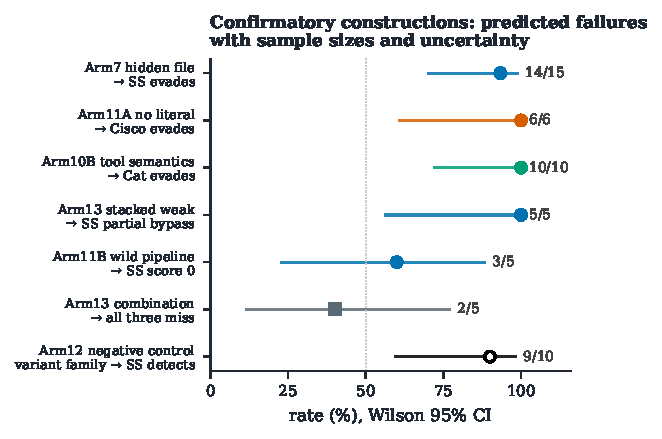
\includegraphics[width=0.62\textwidth]{fig_validation.pdf}%
\Description{Forest plot of seven hypothesis outcomes with Wilson intervals; the negative control is an open marker.}
\caption{\textbf{Confirmatory constructions as rates with uncertainty.} Each row is one locked hypothesis from Table~\ref{tab:cases}; points are observed evasion rates (filled) or, for the negative control, the detection rate (open); bars are Wilson 95\% intervals; $n$ at right. The negative control (Arm12: expanding the best single bypass into a 10-variant family) shows SkillSpector detecting 9/10; single-sample evasion is not family-level evasion, which disciplines every positive row.}
\label{fig:validation}
\end{figure*}

\subsection{A Representative Case, End to End}
The hidden-file hypothesis is the ledger's cleanest full traversal: bottom-up evidence, one locked prediction, one construction family, three different failure layers.
\emph{Derived from (bottom-up):} SkillSpector's build-context source skips dotfiles; Cisco's is-safe rule keeps CRITICAL/HIGH only; the regex engine matches lexical markers only.
\emph{Locked prediction:} payloads placed entirely in hidden files (\texttt{.env}, \texttt{.profile}) evade SkillSpector's analysis.
\emph{Construction:} 15 skills whose SKILL.md is a benign ``environment inspector''; the bundled \texttt{.env} (a shell script despite its name) collects cloud keys, base64-encodes them, and exfiltrates them via \texttt{curl}.
\emph{Validation:} \textbf{14/15 evade} SkillSpector (score $\le$50; 11 exactly 0); Cisco detects 4/15; Caterpillar 2/15.
\emph{Mechanism (Fig.~\ref{fig:oneload}):} SkillSpector's raw output records the analyzed components as exactly \texttt{['SKILL.md']}; the dotfile never entered analysis. The other two fail at different layers on the same samples (Fig.~\ref{fig:oneload}): one artifact, three layers.



\subsection{Role of the Exploratory Arms}
Arms~1--6 ran outside the locking protocol and serve two feasibility roles only: they showed that detectability tracks the operational \emph{surface}: direct \texttt{eval} is caught everywhere, indirect construction is missed by Cisco. They also calibrated the generator (semantic re-wrapping of descriptions changes nothing at SkillSpector, whose evidence comes from code; false capability declarations are counterproductive, tripping the description-code contradiction detector).



% ============================================================
\section{Implications and Future Work}
\label{sec:implications}

\emph{For scanner evaluation.} Aggregate recall is misleading; evaluation should be coordinate-aware, reporting coverage per coordinate.

\emph{For the skill ecosystem.} Single-scanner governance inherits that scanner's blind spots wholesale. In the 581-skill corpus, no all-scanner miss survived sanitization (10 flagged-by-none candidates, each attributed to data-quality, scanner-failure, or threshold artifacts). Locked construction nonetheless found the exception class: stacking independently weak mechanisms evaded all three scanners on 2/5 samples; defense-in-depth fails at the conjunction, not at any single mechanism. Conversely, each scanner has a family where its shipped detection collapses: hidden files for SkillSpector (14/15 evade), finding-specialized variants for Cisco (6/6), and no-literal semantics for the regex tool (10/10).

\emph{For adversarial methodology.} Hypothesis locking separates genuine prediction from post-hoc rationalization and should become standard practice.

\emph{For scanner design and evaluation methodology.} The decomposition says which kind of fix each blind spot admits: SkillSpector's dotfile skip is a coverage defect (include hidden files); Cisco's threshold swallowing is a reporting defect (surface MEDIUM findings: 88 of 581 malicious skills are \texttt{is\_safe} despite MEDIUM-or-higher); the regex engine's no-literal blindness is an architectural limit, not a bug. And three measurement traps had to be corrected before any conclusion was stable: threshold swallowing, technical failures indistinguishable from misses, and ground-truth leakage through provenance metadata; benchmarks that do not control for these mis-report detection.

\emph{Future work.} We are extending this into a full benchmark and a taxonomy-guided defensive filter, to be reported in an extended version. Beyond agent skills, the same loop applies wherever multiple automated analyses judge the same artifact: package registries, dependency scanners, static analyzers, LLM-based security evaluators. Its preconditions are explicit: the threat space must be enumerable into dimensions, and each analysis must expose inspectable outputs (categories, findings, rules) to project. A regex tool with no category system, like our lower-bound reference, cannot be projected at all. Where those hold, the settings already produce disagreement; what they lack is the instrument to read it.

\vspace{\medskipamount}
\noindent\textbf{Takeaway.} Disagreement among security analyses is usually filed as an evaluation inconvenience. Read structurally, it is a map of what each analysis cannot see, and that map can be drawn before an attacker walks it.

% ============================================================
\section{Related Work}
\label{sec:related}

Prior work addresses individual parts of this problem. Malicious-skill benchmarks~\cite{malskillbench2026,skilltrustbench2026} label corpora along their own taxonomies; we instead map \emph{scanner outputs} onto a coordinate space to interrogate disagreement. Scanner evaluations~\cite{clawhub2026,locatejudge2026,skillscan2026,skillsmetric2026} quantify disagreement or recall without structural attribution; SkillsMetric maps one self-built framework's boundary, while we analyze production scanners and predict failures before constructing them. Adversarial generation~\cite{cloakdetonate2026,colluskill2026} shows evasion is possible (over 90\% on eight scanners; 96\% on six) but searches generically; our constructions derive from locked hypotheses about \emph{where} each architecture fails, with misses traced to source level. Implementation audits such as SkillProbe~\cite{skillprobe2026} formalize declaration-inconsistency within one framework; ours connects implementation properties to a cross-scanner attack model. Our contribution connects these steps into a single analysis loop.

% ============================================================
\bibliographystyle{ACM-Reference-Format}
\bibliography{references}

\end{document}
